\section{EVALUATIE}
\label{chap:Evaluation}

Om de doeltreffendheid te meten van dynamische windowing voor multi-stream operatoren tijdens de 
mapping van niet-RDF heterogene gegevens moeten we de volgende 
metrieken van ons stream processing framework: \emph{CPU gebruik}, \emph{latency}, \emph{doorvoer},
\emph{geheugengebruik}, en \emph{compleetheid}. 

\subsection{Gegevens}
We gebruiken dezelfde gegevens 
als de benchmark in het artikel van Van Dongen en Van den Poel~\cite{evalution_of_spe}. 
De gegevens zijn afkomstig van de NDW (Nationale Databank Wegverkeersgegevens) uit 
Nederland~\footnote{NDW-datasite: \href{http://opendata.ndw.nu/}{http://opendata.ndw.nu/} }.
Het bestaat uit metingen van het aantal auto's en hun gemiddelde snelheid over de verschillende 
rijstroken op een snelweg. 
De sensorgegevens werden door een Kafka-publisher naar twee topics doorgespeeld, namelijk 
\emph{ndwflow} en \emph{ndwspeed}, voor respectievelijk het aantal auto's en de gemiddelde snelheid.

\subsection{Evaluatie setup}

Docker\footnote{Docker: \url{https://www.docker.com}} is 
opgezet met de containers 
zoals ge\"illustreerd in figuur~\ref{fig:docker_setup}. De docker-containers 
draaien op een standalone machine om de invloed van 
netwerkcommunicatie zo veel mogelijk te beperken. Apache Kafka wordt gebruikt 
als de berichtenmakelaar voor onze gegevens. De setup voor de Kafka broker is 
hetzelfde als beschreven in \cite{evalution_of_spe}. 



\begin{figure}[htpb]
    \centering
    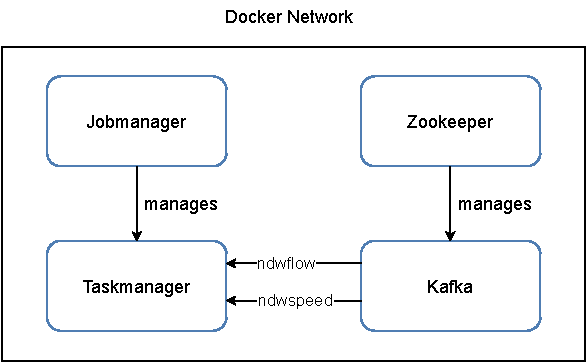
\includegraphics[width=\columnwidth]{fig/docker_setup.pdf}
    \caption[Setup of application containers inside the same docker network.]{ 
Setup van applicatiecontainers binnen hetzelfde docker netwerk.
De kafka topics \emph{ndwflow} en \emph{ndwspeed} worden verbruikt door de 
RMLStreamer job binnen de Taskmanager.}
    \label{fig:docker_setup}
\end{figure}

\subsection{Metingen}%
\label{sub:Metrics measurement}

CPU-gebruik, doorvoer, geheugen, en latency blootgesteld 
door Flink's Rest API, worden constant elke 100ms opgevraagd door een 
Python script scraper.
CPU gebruik, doorvoer 
en geheugengebruik worden intern gemeten door Flink,
terwijl latency meting 
handmatig wordt ge\"implementeerd met behulp van Flink's Metrics API om nauwkeuriger de hoeveelheid tijd te meten 
tijd die een record in het venster doorbrengt voordat het verwerkt wordt. 

De bovengenoemde metrieken worden gemiddeld over de geparallelliseerde window operators.
Intersection over union (IOU) wordt gebruikt als de metriek om de volledigheid te meten
van het samengevoegde resultaat dat door de vensters wordt gegenereerd.  


\subsubsection{CPU-gebruik}%
\label{ssub:CPU usage}
Voor CPU-gebruik meten we het CPU-gebruik van Taskmanager, aangezien die 
verantwoordelijk is voor het uitvoeren van de RMLStreamer-code. 

\subsubsection{Doorvoer}%
\label{ssub:Throughput}
De doorvoermeting wordt gedefinieerd als het aantal records dat per seconde door de 
vensteroperator per seconde. 
Deze wordt gemeten aan de uitvoer van de window operator, aangezien we de 
uitvoerprestaties van de windowoperators willen meten. 


\subsubsection{Geheugengebruik}%
\label{ssub:Memory usage}
Vanwege de beperking in granulariteit van metingen in Flink, 
JVM heap geheugen van de job gebruikt om het geheugengebruik van de window 
operator. We verwachten dat het geheugengebruik door andere operators in de job 
consistent en laag is over de verschillende evaluatieruns, omdat het stateless operators zijn.

\subsubsection{Latency meting}%
\label{ssub:Latency measurement}
We meten de latentie door een tijdstempel toe te voegen aan de 
records voordat ze het venster binnenkomen. 
Zodra de records verwerkt zijn en na de join worden uitgezonden, wordt het verschil 
tussen de huidige verwerkingstijd en de bijgevoegde oude verwerkingstijd 
genomen als de \emph{latency} voor de records. 

\subsubsection{Voltooidheidsmeting}%
\label{ssub:Completeness measurement}
Om \emph{begrensde} invoergegevens te genereren voor 
de static mapping engine, schrijven we de opgeslagen gegevens van de topics 
in een bestand op schijf. Deze invoergegevens worden door RMLStreamer verwerkt in de modus voor 
verwerkingsmodus om de \emph{complete} set triples te genereren. 

De gegenereerde output triples van de evaluatie van de vensters en de verwerking van de begrensde gegevens worden 
gebruikt om de IOU-metriek te berekenen om de gelijkenis tussen de twee outputs te meten.    



\subsection{Werklastscenario's}
\label{sec:workload}
We evalueren onze dynamische vensterimplementatie onder verschillende werklastscenario's. 
Deze werklasten zijn vergelijkbaar met die welke in~\cite{evalution_of_spe} zijn gebruikt, voor zover relevant.

\subsubsection{Werklast voor latentiemeting}
Meting van de \emph{latency} die alleen wordt veroorzaakt 
door de vensterimplementaties, vereist dat het stroomverwerkingsraamwerk niet wordt 
door aanzienlijke \emph{doorvoer} wordt belast. Dus, de Kafka makelaar 
de records op een zeer lage constante snelheid van ongeveer 400 berichten per seconde voor 
deze werklast.
We noemen dit in de paper \emph{constant} stream rate. 

\subsubsection{Werklast met periodieke burst}
We evalueren onze implementatie op zijn vermogen om te gaan met onstabiele 
streaming gegevensbronnen met variërende snelheid.
De werklast heeft een constante lage streamsnelheid met af en toe een 
uitbarsting van gegevens. Daarom worden elke 10 seconden 38 000 records gepubliceerd, wat 
ongeveer 170 tot 180 ms duurt, aangezien de tijd die nodig is om te publiceren kan afwijken op basis van de 
last van de Kafka-brokers.
We duiden dit in de paper aan als \emph{periodic} stream rate. 

\subsubsection{Werklast voor de volledigheid}
We zullen twee stream rates gebruiken, constant en periodiek, 
om de \emph{compleetheid} te meten van de resultaten gegenereerd 
door de verschillende vensters.






